\chapterA{Introducción}

\section{?`Qué es GIT?}

GIT es un sistema de control de versiones que nos permite gestionar código y sus diferentes versiones a lo largo de una producción. En concreto al hablar de GIT estamos hablando de un sistema de control de versiones \textbf{descentralizado o distribuido}. Esto significa que cada usuario tendrá su propio repositorio y podrán intercambiar y mezclar versiones entre ellos. Normalmente habrá un repositorio central que sirva de sincronización entre los distintos usuarios.

\section{Pack de estudiantes de GitHub}

Las ventajas principales del pack de estudiantes son:
\begin{itemize}
    \item Repositorios privados ilimitados.
    \item Herramientas disponibles solo para repositorios públicos (gráficos de contribución, ramas protegidas, GitHub Pages, etc) en repositorios privados.
    \item Cursos ofrecidos por otras compañías.
\end{itemize}

Para conseguir estas ventajas solo hay que ir a \url{https://education.github.com/} y registrarte con la cuenta de correo de la universidad.

En caso de que ya tengas cuenta con otro correo, inicia sesión como lo harías normalmente, ve a la página \url{https://github.com/settings/emails} y añade un correo adicional.

\section{Creación de un repositorio}

\begin{figure}[ht]
    \begin{minipage}{0.3\linewidth}
        \centering
        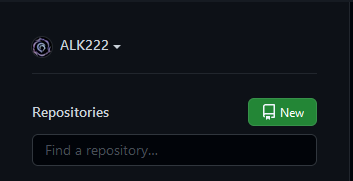
\includegraphics[width=0.9\linewidth,]{creacion_repo.png}
        \caption{Botón de creación de repositorio}
        \label{fig:crea_repo}
    \end{minipage}%
    \begin{minipage}[b]{0.7\linewidth}
        \setlength{\parindent}{0.2in}

        Para crear un repositorio nuevo iremos a la página principal (\url{https://github.com}) y buscaremos en la parte superior derecha el botón verde de creación.

        Tras esto, se nos ofrecerán una serie de opciones a la hora de crearlo, como si queremos que sea público o privado, el nombre del mismo, o las opciones de licencia, \textit{readme} y \textit{gitignore}.
    \end{minipage}
\end{figure}

Estas opciones son:
\begin{itemize}
    \item\textbf{Nombre del repositorio:} se explica por sí solo. Será el nombre de la carpeta al clonarla en nuestro PC. Conviene sustituir los espacios en blanco por guiones o barras bajas.
    \item\textbf{Descripción:} Resumen del objetivo del repositorio, opcional.
    \item\textbf{Público/Privado:} Puedes escoger si el resto de gente puede ver tu repositorio o no. Esto se puede cambiar tras la creación del repositorio en cualquier momento.
    \item\textbf{README:} archivo donde das una información mas detallada sobre el repositorio. Normalmente la gente no lo lee.
    \item\textbf{.gitignore:} archivo que va a determinar que archivos \textbf{no} se suben al repositorio. Puede editarse a mano, pero los predefinidos para cada lenguaje por github están bastante completos.
    \item\textbf{Licencia:} establece las condiciones de uso del resto de usuarios.
\end{itemize}

\section{Añadir colaboradores a un repositorio}

Si queremos trabajar con un equipo en un repositorio privado, tendremos que darles acceso al mismo. Para este ejemplo usaremos un usuario de nombre \textit{A} que tiene un repositorio de nombre \textit{prueba}.

Para añadir gente a \textit{prueba} podemos ir a la propia página del repositorio desde nuestro perfil, debajo de la barra vista en \ref{fig:crea_repo}~(\nameref{fig:crea_repo}) y buscarlo ahí.

Una vez entremos en la página del repositorio podemos ir a la configuración del mismo en la barra que tendremos justo debajo del nombre del repositorio.
Para hacerlo de forma más directa, iríamos a \url{https://github.com/A/prueba}.

Una vez en la configuración iremos a \textbf{collaborators}. Una vez en esa pestaña se nos pedirá nuestra contraseña para continuar. Después de introducir la contraseña buscaremos el botón verde de \textbf{add people} y podremos buscarles por nombre de usuario o correo.

Para que los usuarios invitados tengan acceso, deberán seguir los pasos que se nombran en el correo que les llegará a su correo principal de GitHub.
